\documentclass[aspectratio=169]{beamer}
\usepackage[utf8]{inputenc}
\usepackage[T1]{fontenc}

\usepackage{theme/beamerthemeNBersp}


\title{Modulación de fase en ondas de Faraday}
\subtitle{Laboratorio 6 y 7}
\author{
	Bernardo Español \and Melisa Vinograd
	\texorpdfstring{\\ \vspace{0.1cm} Dirección: Dr. Pablo Cobelli}{}
}
\institute{Laboratorio de Turbulencia Geofísica, FLiP: Fluidos y Plasmas}
\date{} 

\begin{document}

% Título
\begin{frame}[noframenumbering,plain]
	\titlepage
\end{frame}

\begin{frame}{Índice}
	\tableofcontents
\end{frame}


\section{Motivación}

\begin{frame}{Ondas de Faraday} % TODO
	\begin{figure}[ht]
		\centering
		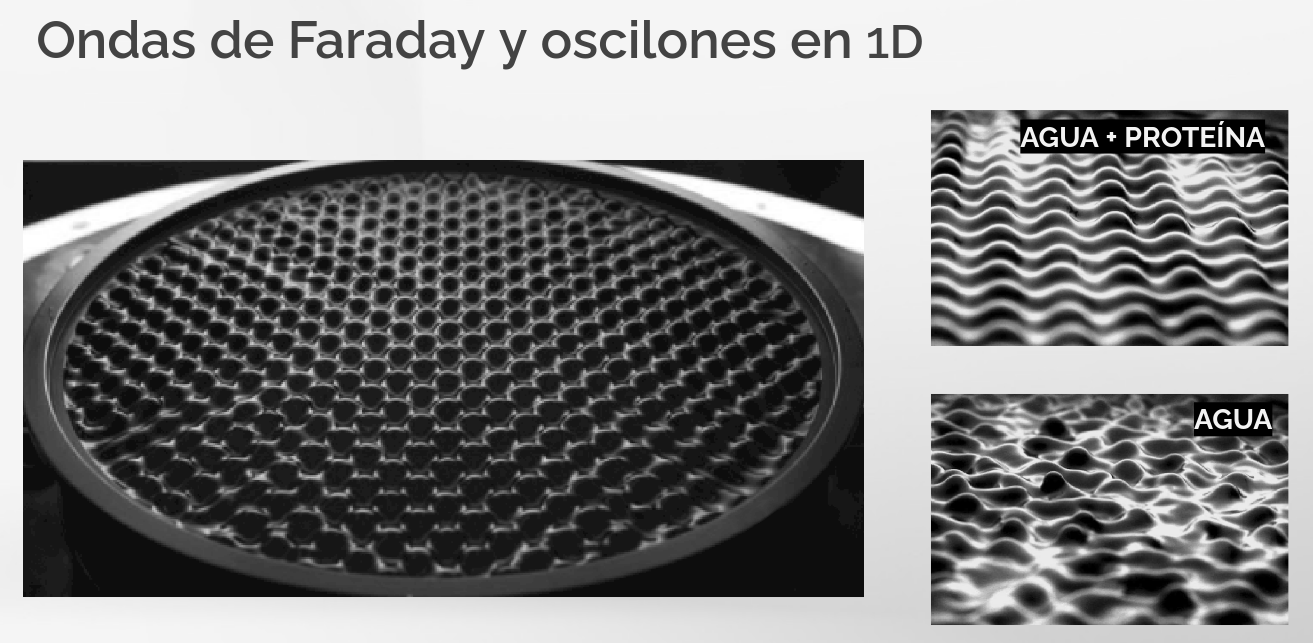
\includegraphics[width=1\textwidth]{figs/ss1.png}
	\end{figure}
\end{frame}

\begin{frame}{Oscilones en 1D} % TODO
	\begin{figure}[ht]
		\centering
		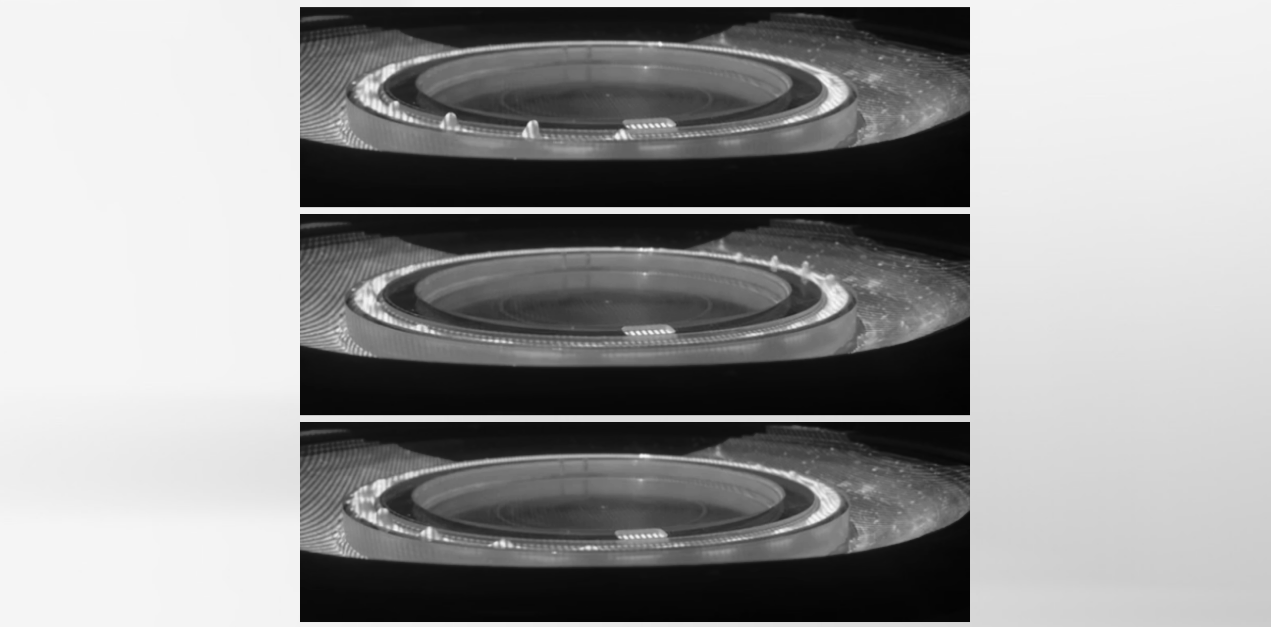
\includegraphics[width=1\textwidth]{figs/ss3.png}
	\end{figure}
\end{frame}

\section{Montaje experimental}

\begin{frame}{Montaje experimental}
	\begin{figure}[ht]
		\centering
		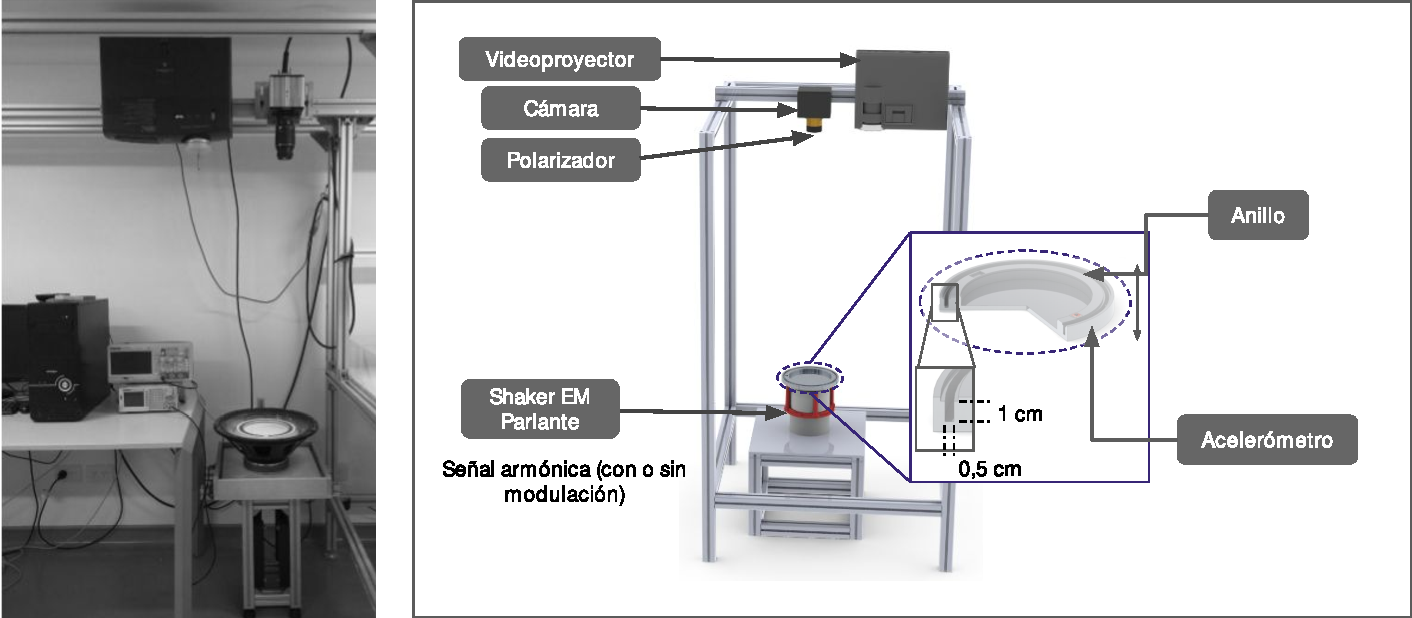
\includegraphics[width=1\textwidth]{figs/esquema_experimental.pdf}
	\end{figure}
\end{frame}

\section{Extracción de la superficie libre}

\begin{frame}{FTP}
	\begin{minipage}{0.7\textwidth}
	  \begin{figure}
		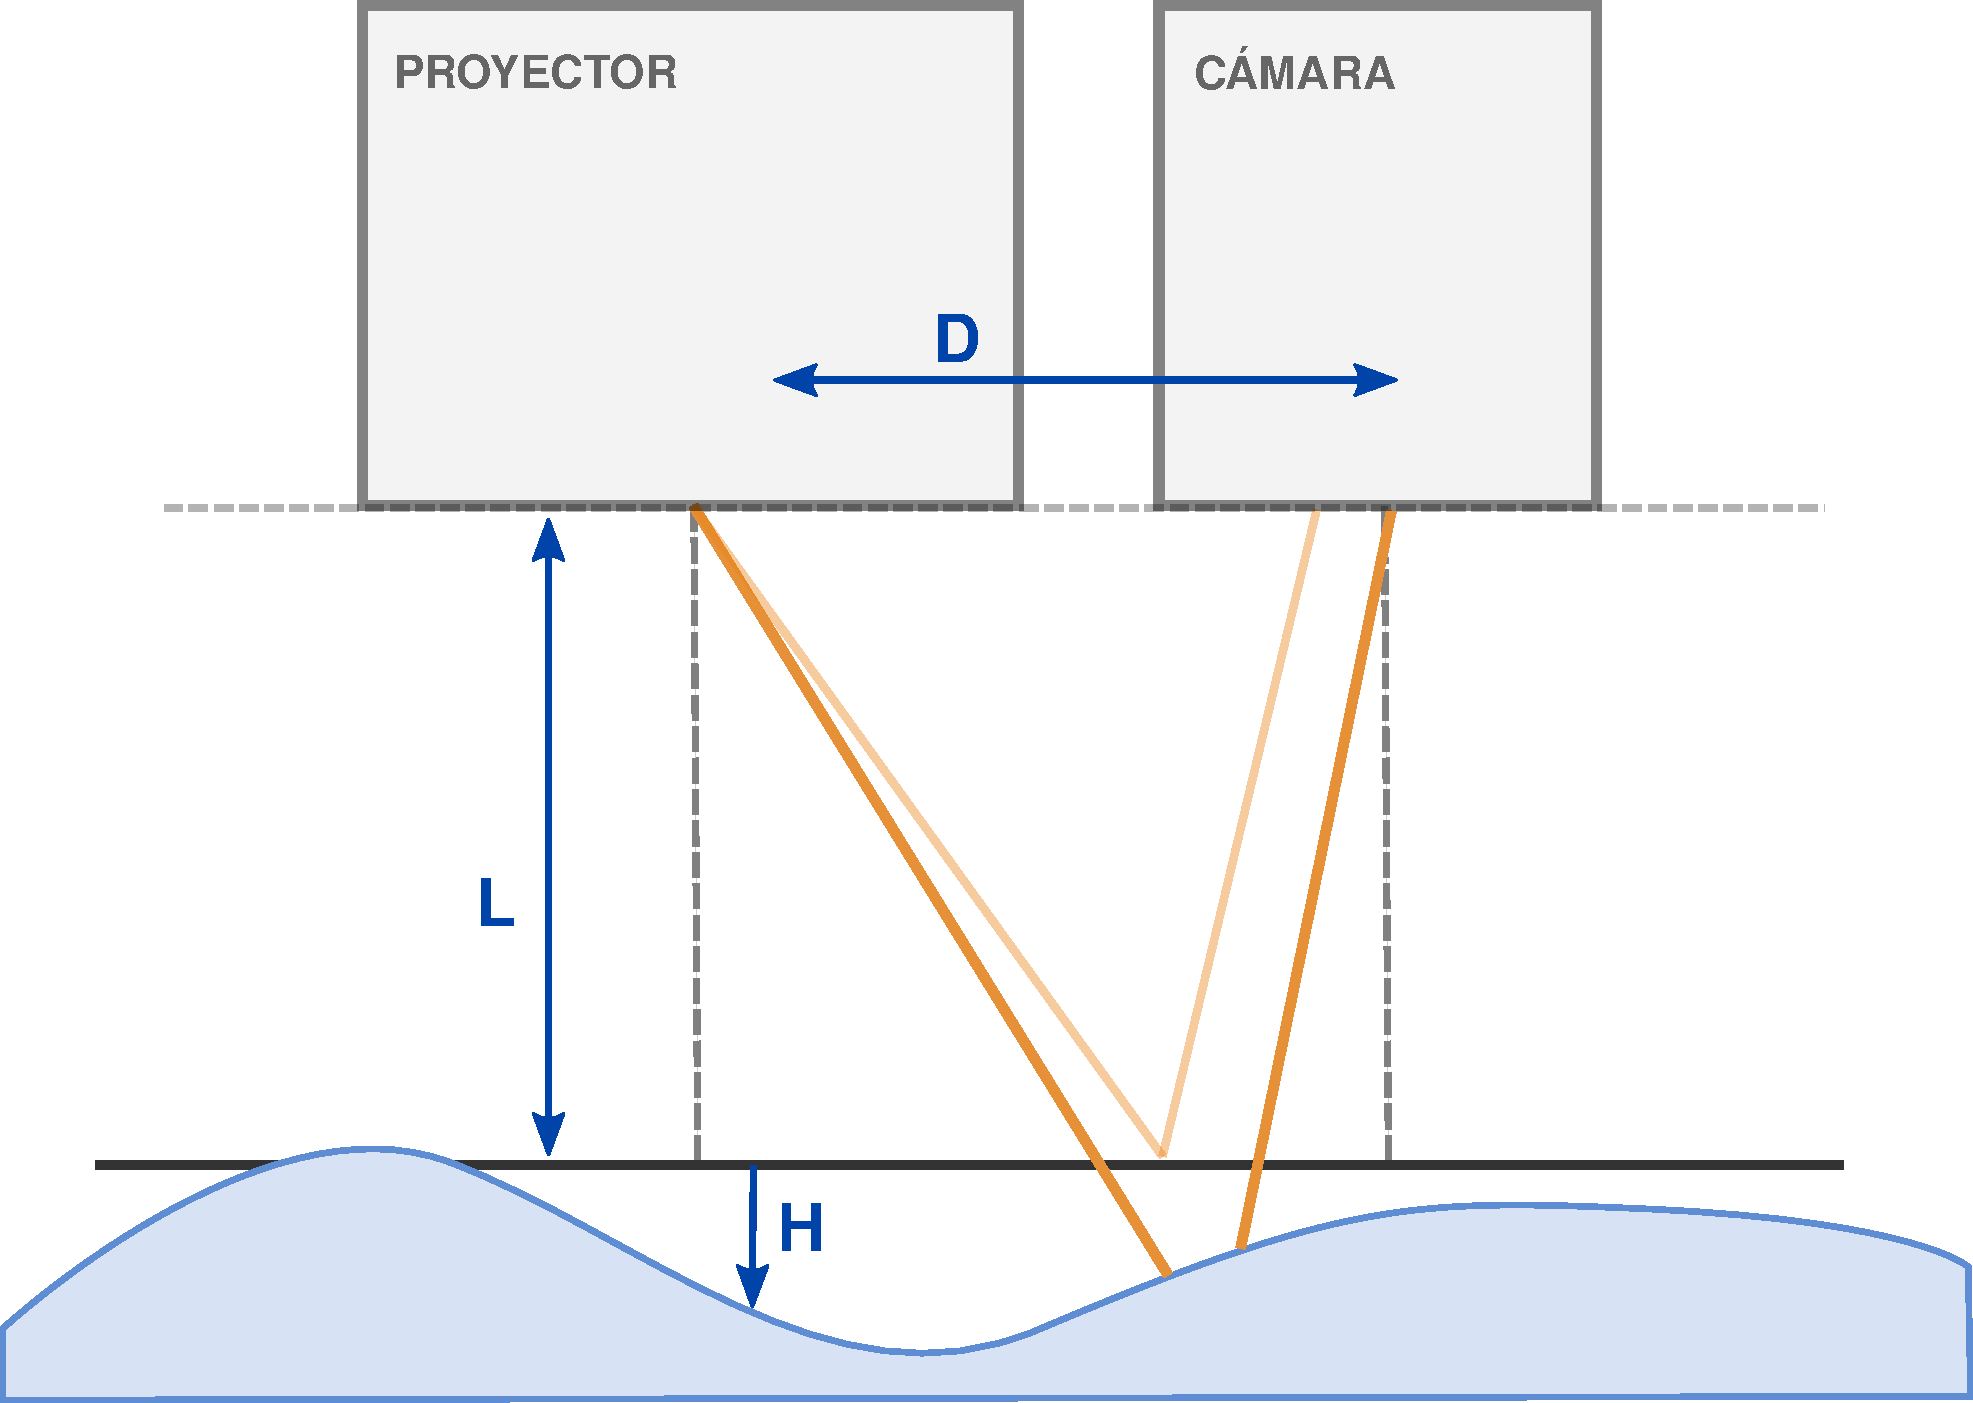
\includegraphics[width=1\textwidth]{figs/ftp_experimental.pdf}
	  \end{figure}
	\end{minipage} \hfill
	\begin{minipage}{0.29\textwidth}
	  \begin{figure}
	    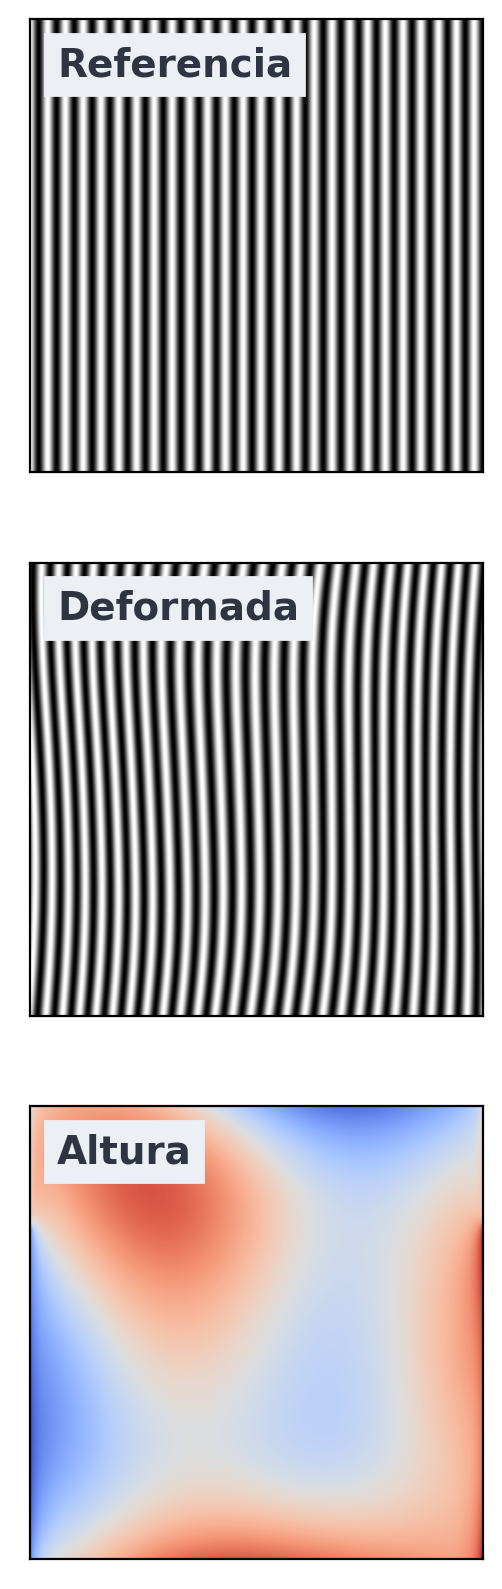
\includegraphics[width=0.56\textwidth]{figs/synthetic_ftp.png}
	  \end{figure}
	\end{minipage}
\end{frame}

\begin{frame}{Extracción de la superficie libre} % TODO (4 diapos)
	\begin{figure}[ht]
		\centering
		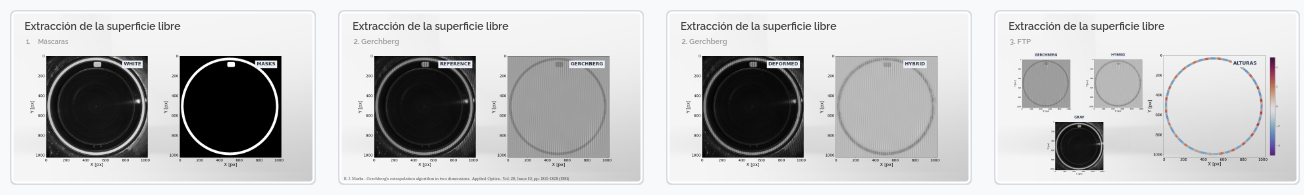
\includegraphics[width=1\textwidth]{figs/ss4.png}
	\end{figure}
\end{frame}

\begin{frame}{Extracción de la superficie libre} % TODO
	\begin{minipage}{0.49\textwidth}
	  \begin{figure}
	    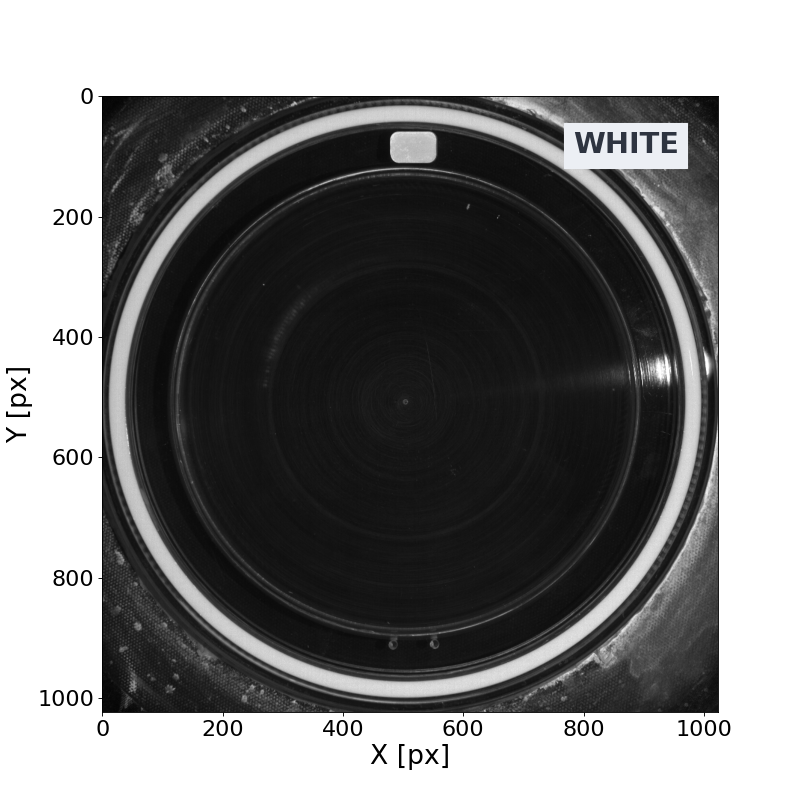
\includegraphics[width=\linewidth]{figs/ftp_white.png}
	  \end{figure}
	\end{minipage} \hfill
	\begin{minipage}{0.49\textwidth}
	  \begin{figure}
	    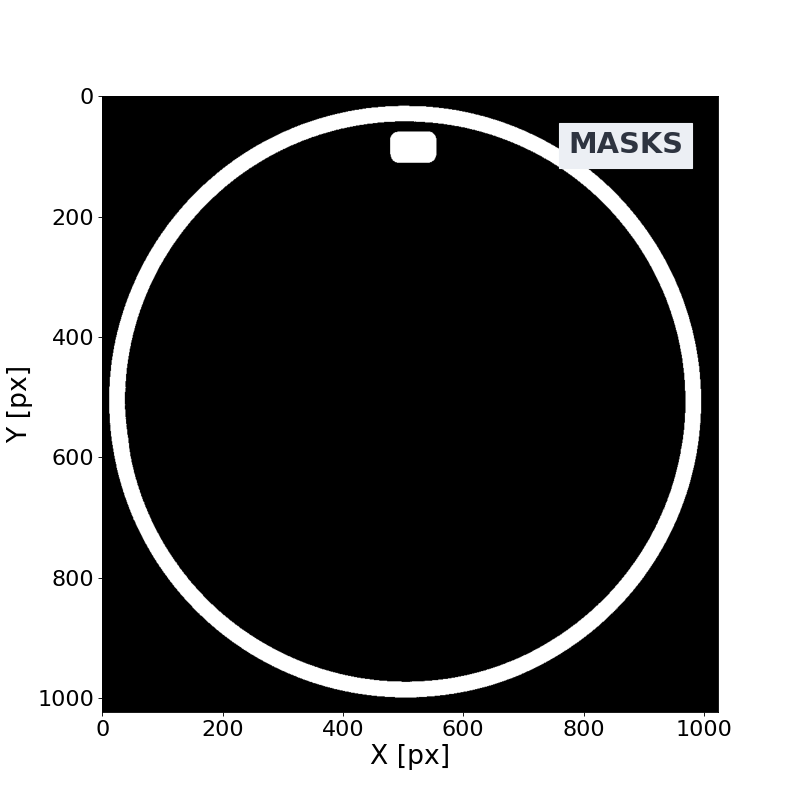
\includegraphics[width=\linewidth]{figs/ftp_masks.png}
	  \end{figure}
	\end{minipage}
	% TODO[meli]: Volver a exportar
\end{frame}

\begin{frame}{Extracción de la superficie libre} % TODO
	\begin{minipage}{0.49\textwidth}
	  \begin{figure}
	    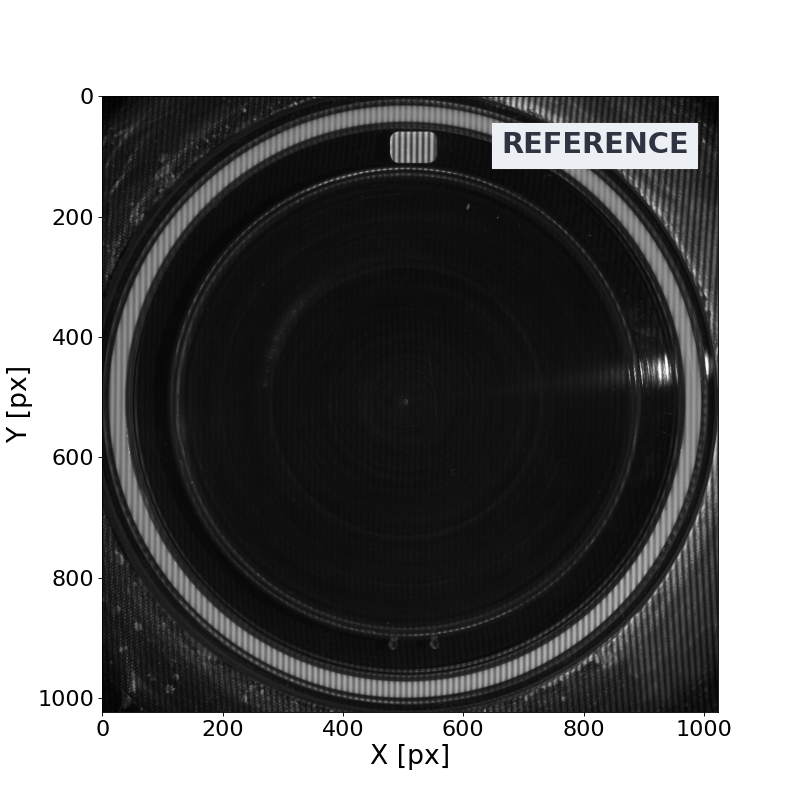
\includegraphics[width=\linewidth]{figs/ftp_reference.png}
	  \end{figure}
	\end{minipage} \hfill
	\begin{minipage}{0.49\textwidth}
	  \begin{figure}
	    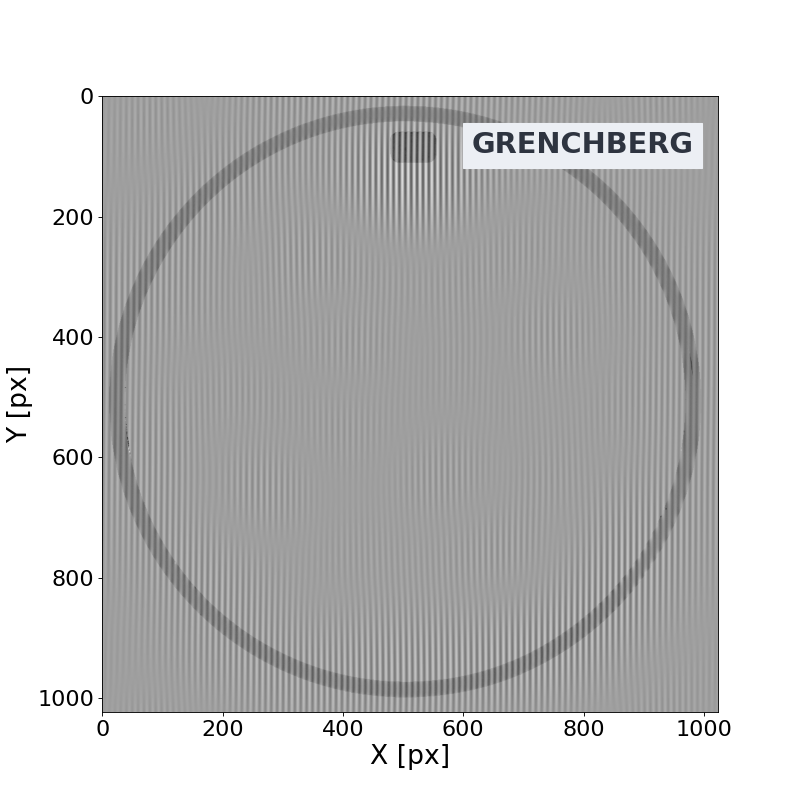
\includegraphics[width=\linewidth]{figs/ftp_gerchberg.png}
	  \end{figure}
	\end{minipage}
	% TODO[meli]: Volver a exportar
\end{frame}

\begin{frame}{Extracción de la superficie libre} % TODO
	\begin{minipage}{0.49\textwidth}
	  \begin{figure}
	    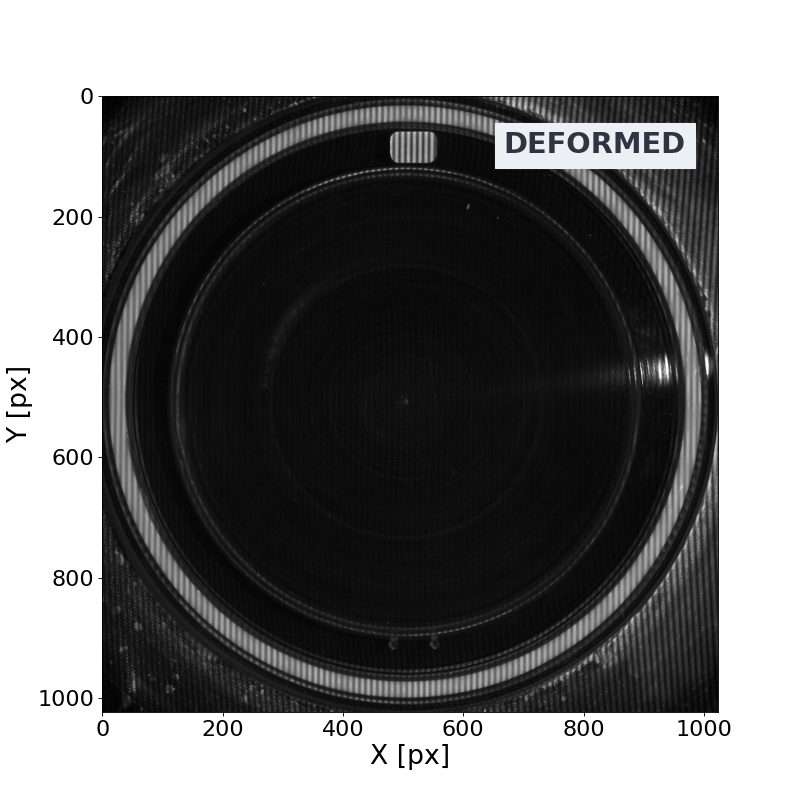
\includegraphics[width=\linewidth]{figs/ftp_deformed.png}
	  \end{figure}
	\end{minipage} \hfill
	\begin{minipage}{0.49\textwidth}
	  \begin{figure}
	    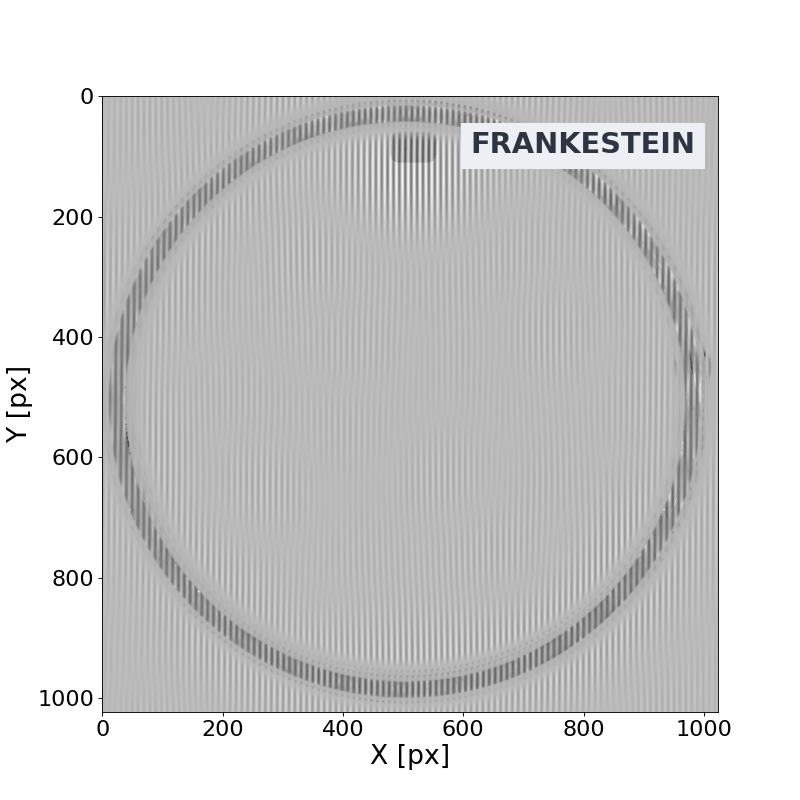
\includegraphics[width=\linewidth]{figs/ftp_hybrid.png}
	  \end{figure}
	\end{minipage}
	% TODO[meli]: Volver a exportar
\end{frame}

\begin{frame}{Extracción de la superficie libre} % TODO
	\begin{minipage}{0.49\textwidth}
	  \begin{figure}
	    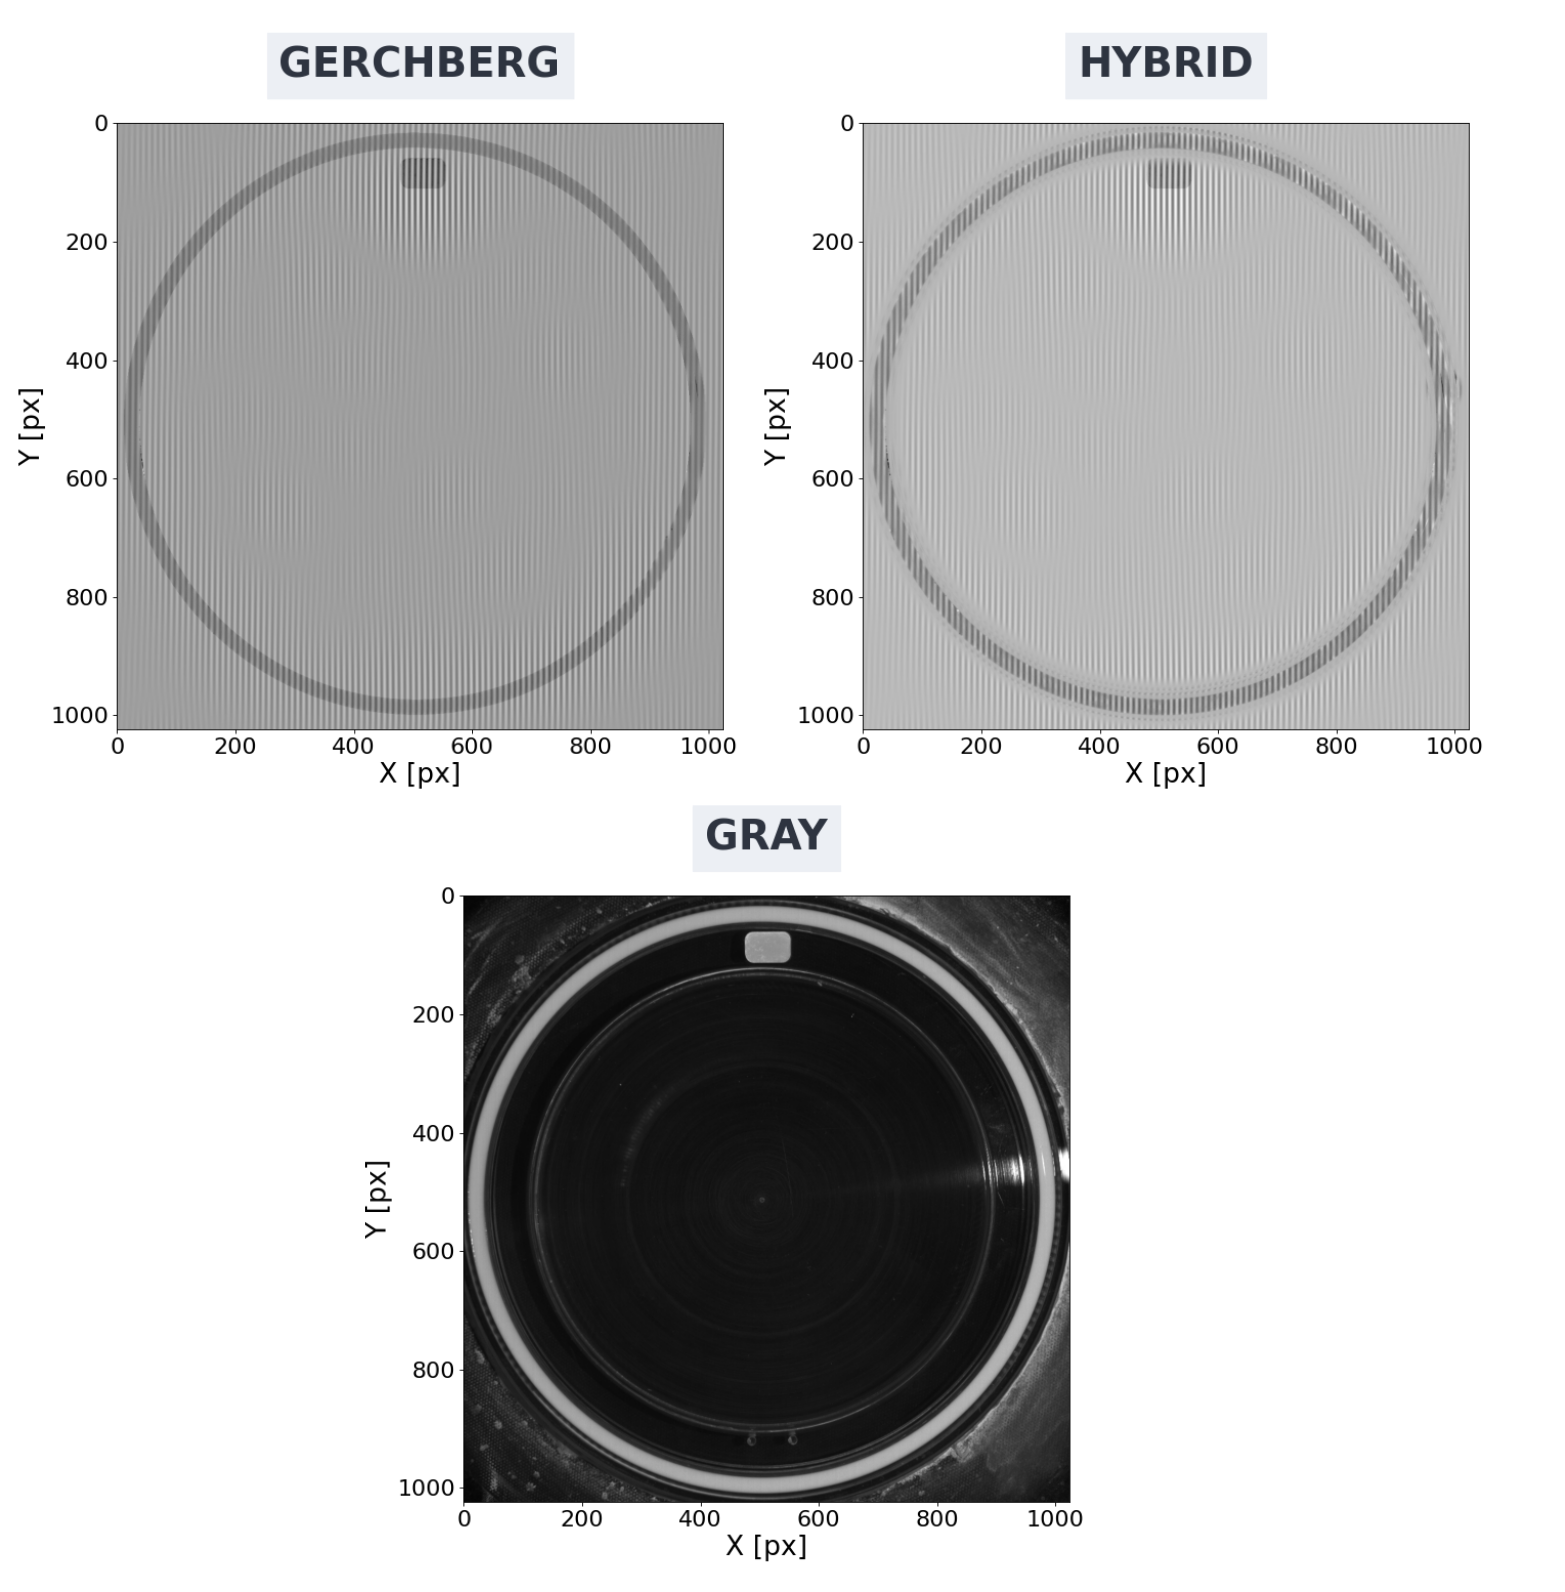
\includegraphics[width=0.85\linewidth]{figs/ftp_collage.png}
	  \end{figure}
	\end{minipage} \hfill
	\begin{minipage}{0.49\textwidth}
	  \begin{figure}
	    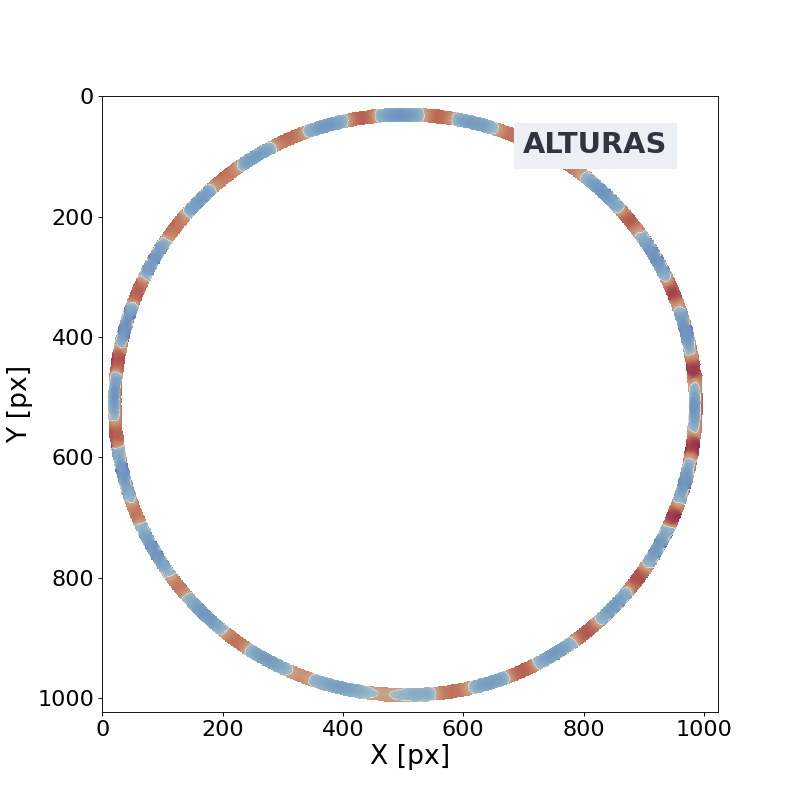
\includegraphics[width=\linewidth]{figs/alturas.png}
	  \end{figure}
	\end{minipage}
	% TODO[meli]: Volver a exportar
\end{frame}


\begin{frame}{Extracción de la superficie libre} % TODO
	\begin{minipage}{0.49\textwidth}
	  \begin{figure}
	    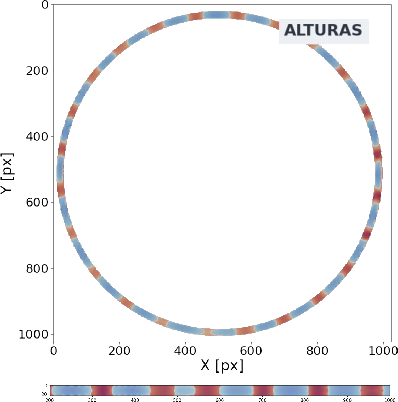
\includegraphics[width=0.8\linewidth]{figs/anillo_a_strip.png}
	  \end{figure}
	\end{minipage} \hfill
	\begin{minipage}{0.49\textwidth}
	  \begin{figure}
	    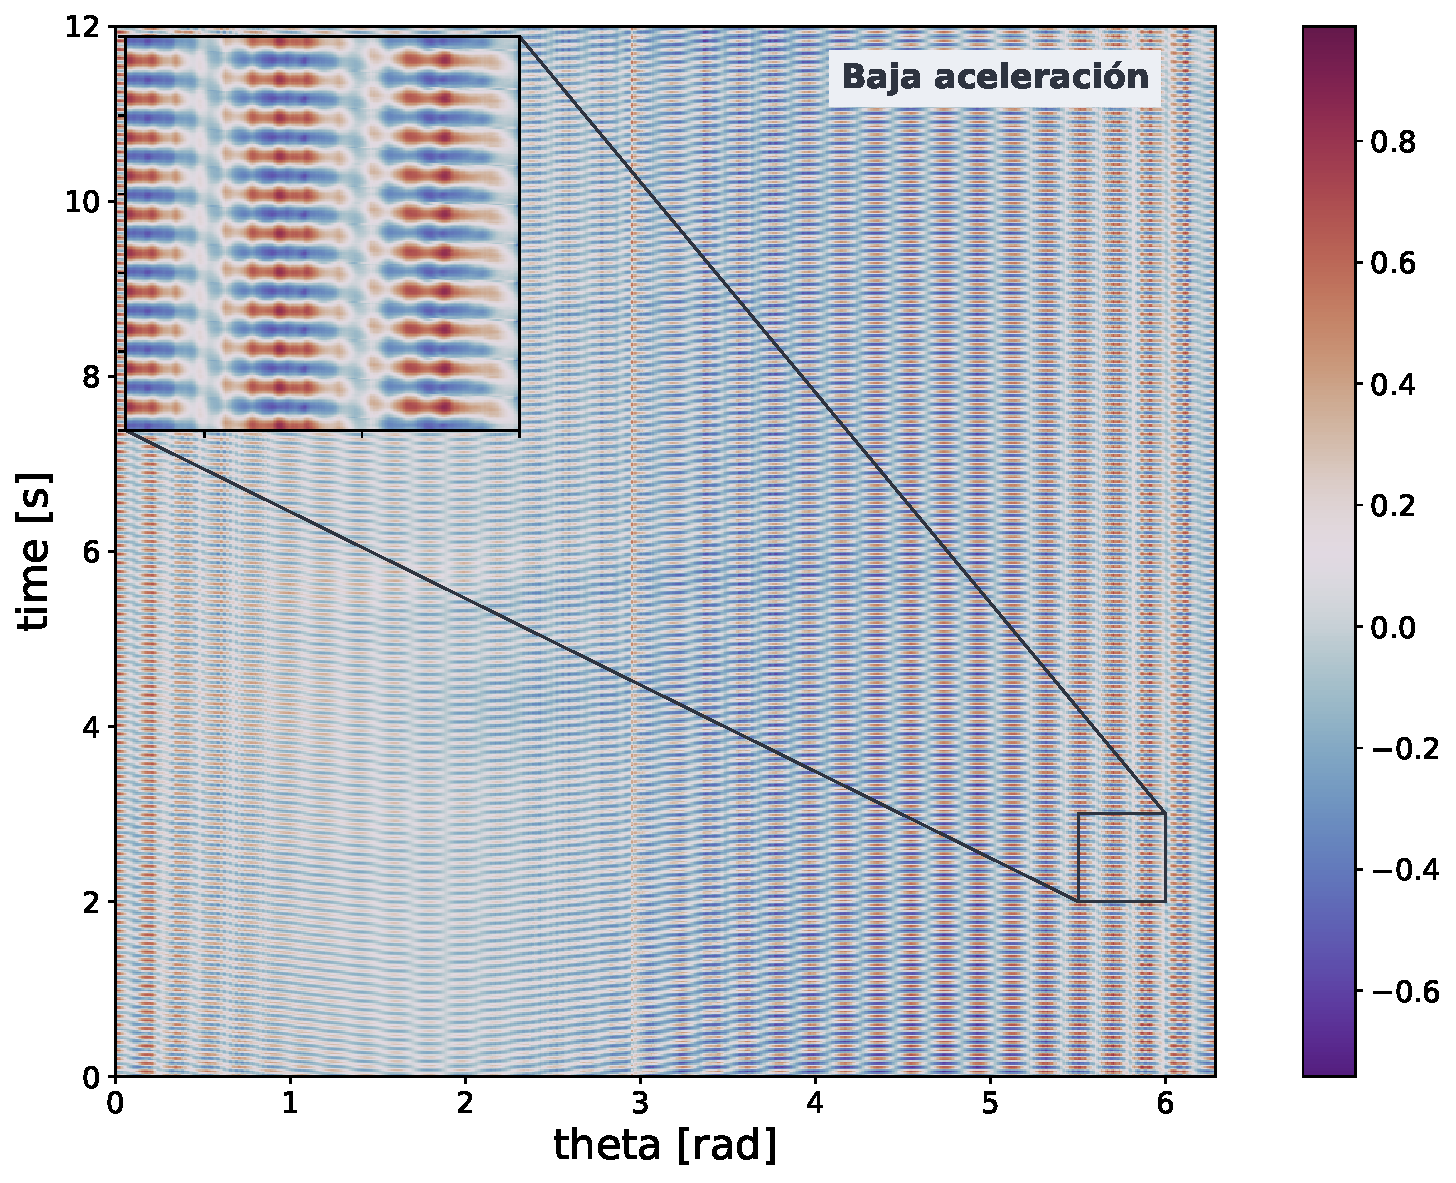
\includegraphics[width=\linewidth]{figs/st_MED5.pdf}
	  \end{figure}
	\end{minipage}
	% TODO[meli]: Volver a exportar
\end{frame}

\begin{frame}{Algunas métricas} % TODO
	\begin{itemize}
		\item 70 mediciones
		\item Videos de $12\text{s}$ de medición a $250\text{fps}$ 
		\item Fotogramas de $(1024\cross1024)\text{px}$
		\item Espacio en memoria 
			\begin{itemize}
				\item $4\text{GB}$ (mediciones crudas)
				\item $40\text{GB}$ (mediciones procesadas)
				\item $100\text{MB}$ (espacio-temporal)
			\end{itemize}
		\item Tiempo de ejecución: $1\text{h} \rightarrow 10\text{min}$
	\end{itemize}
\end{frame}


\begin{frame}{Corrección de errores en los diagramas espacio-temporales}
	\begin{figure}[ht]
		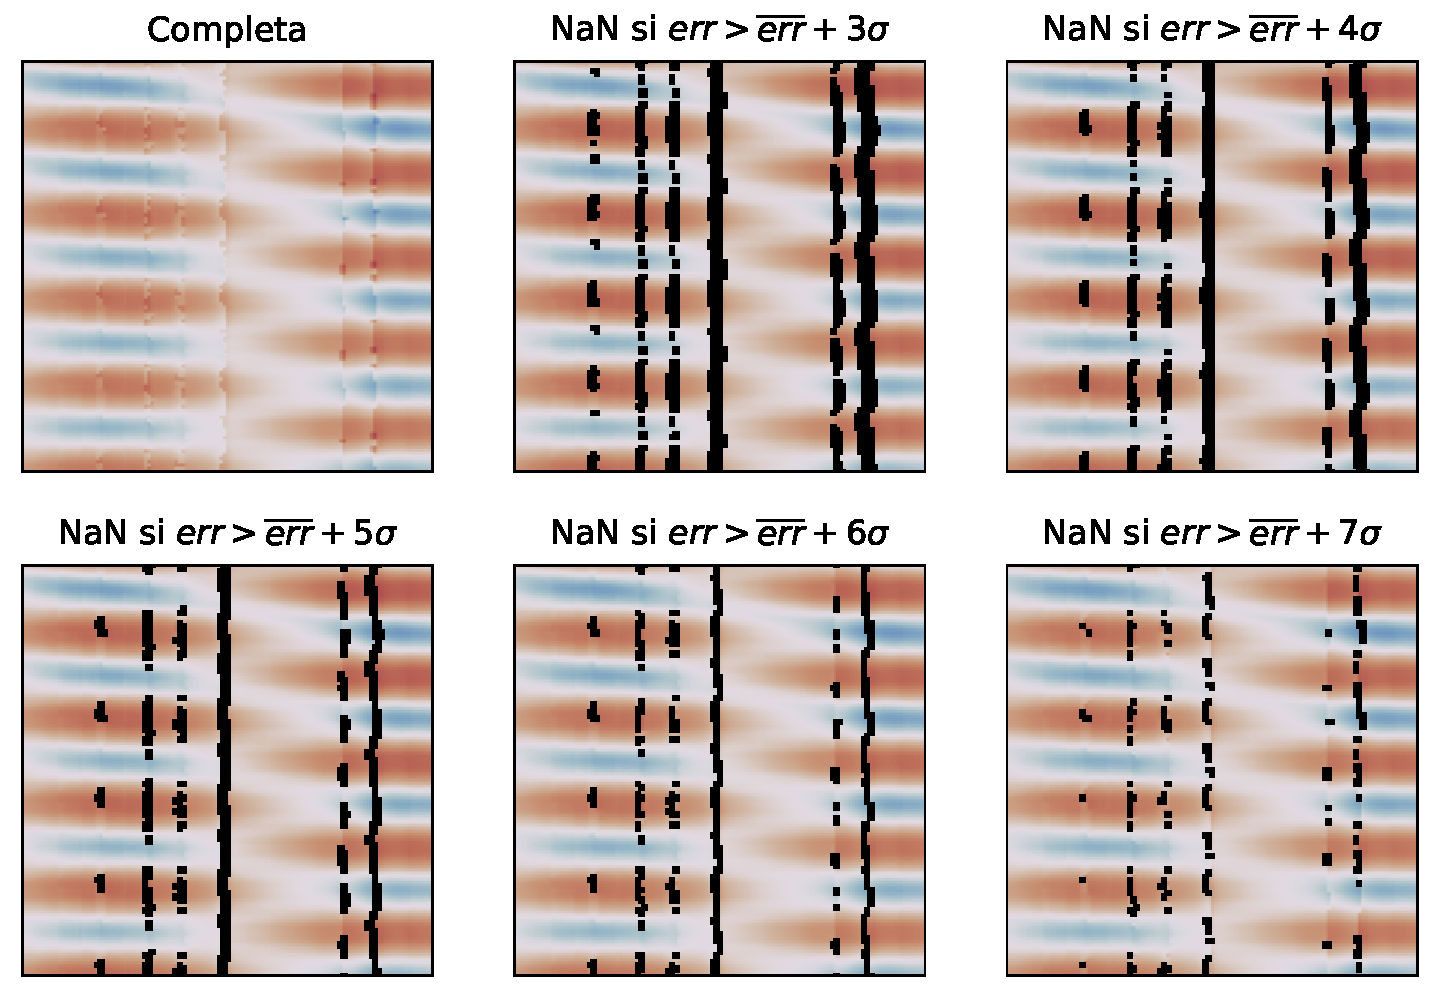
\includegraphics[width=0.75\linewidth]{figs/error_analysis.pdf}
	\end{figure}
\end{frame}

\begin{frame}{Corrección de errores en los diagramas espacio-temporales}
	\begin{figure}[ht]
		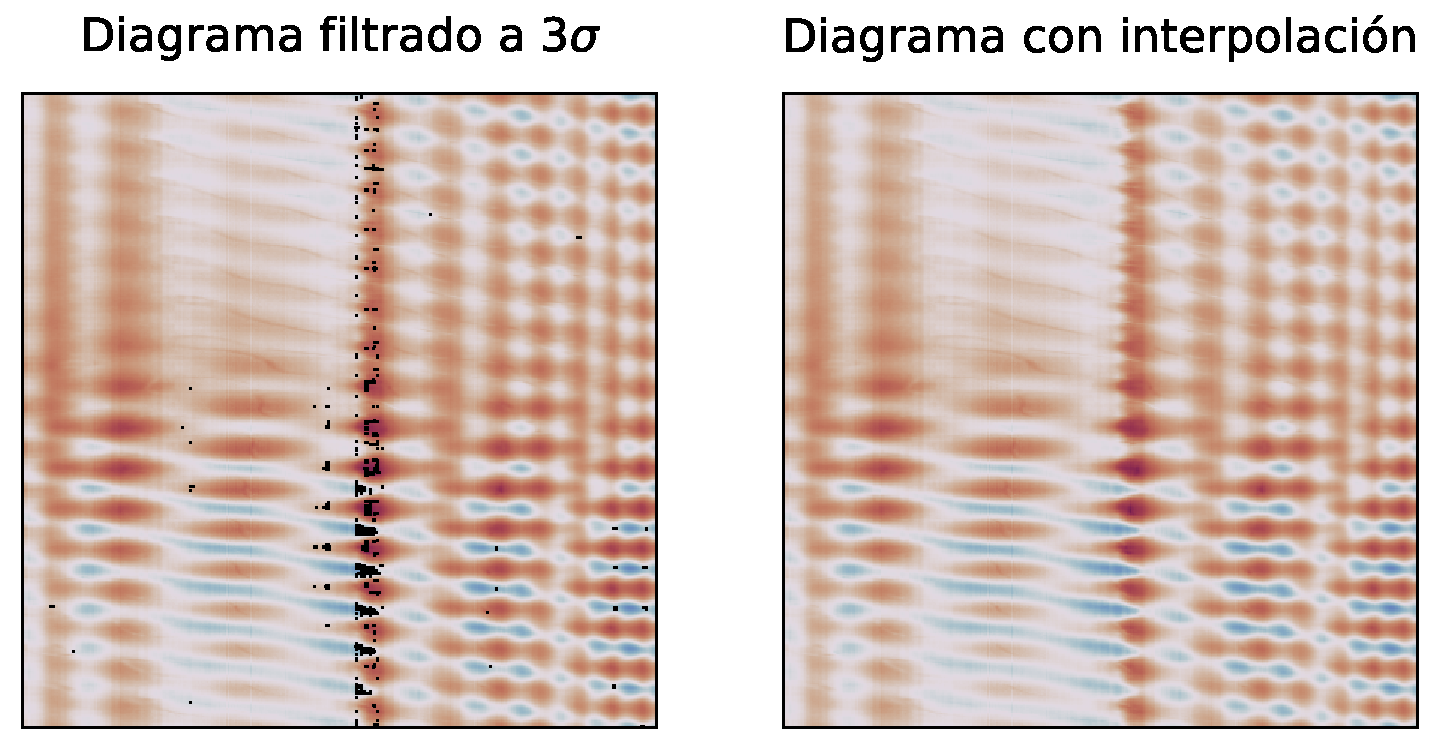
\includegraphics[width=0.8\linewidth]{figs/error_interp.pdf}
	\end{figure}
\end{frame}

\section{Resultados}

\begin{frame}{Zoología de resultados}
	\begin{itemize}
		\item Simple faraday
		\item Expansión/Compresión
		\item Oscilones suaves
		\item Oscilones violentos
		\item Modulación de fase
	\end{itemize}
\end{frame}

\begin{frame}{Ondas propagativas} % TODO: Ponerle alturas?
	\begin{figure}[ht]
		\centering
		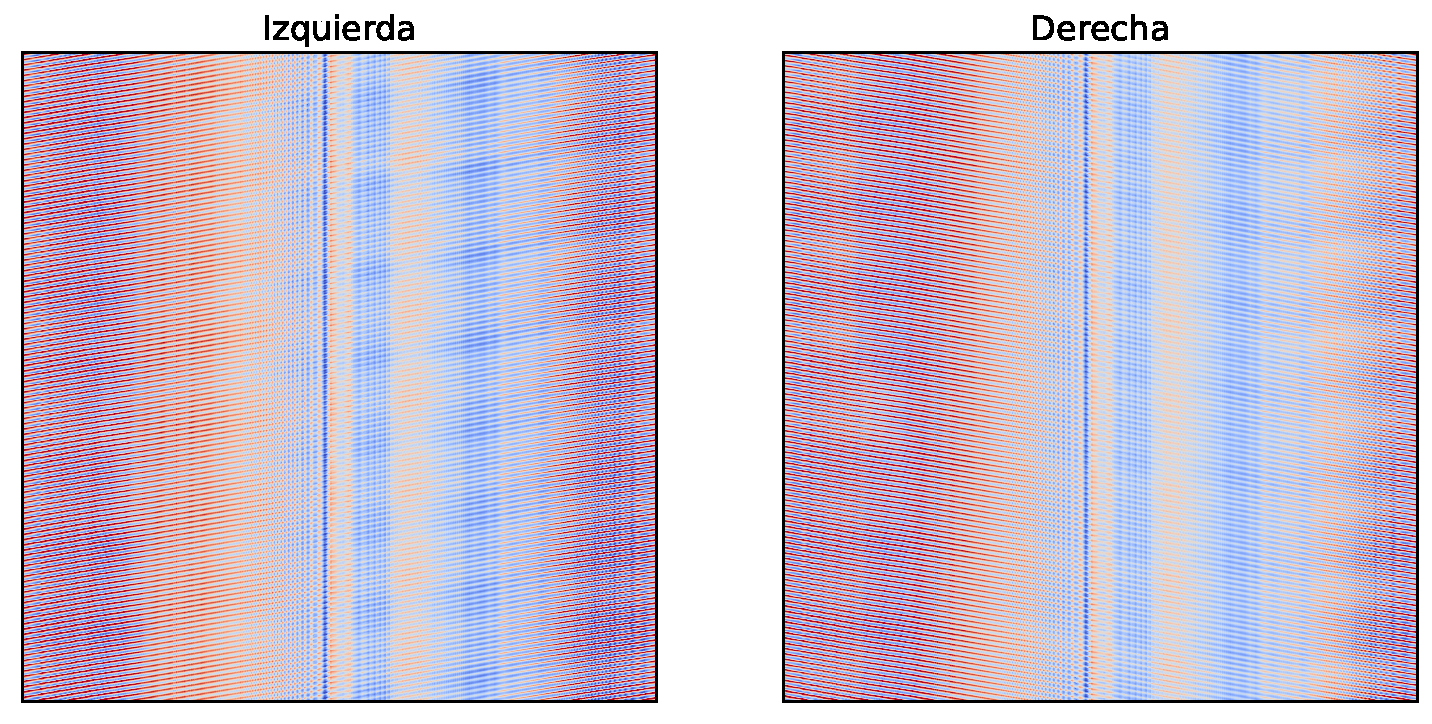
\includegraphics[width=0.8\textwidth]{figs/st_left_right.pdf}
	\end{figure}
\end{frame}

\begin{frame}{Detección de la velocidad de los oscilones} % TODO
	
\end{frame}

\begin{frame}{Ajuste de oscilones} % TODO (2 diapos): Un solo oscilón y todos juntos
	
\end{frame}

\begin{frame}{Relación de dispersión} % TODO: Las que vimos lineales y ver las de modulación de fase
	
\end{frame}

\begin{frame}{Inestabilidad de Taylor-Couete} % TODO
	
\end{frame}


\begin{frame}{Envolvente de la superficie libre} % TODO: Quizás otra diapo?
	\begin{figure}[ht]
		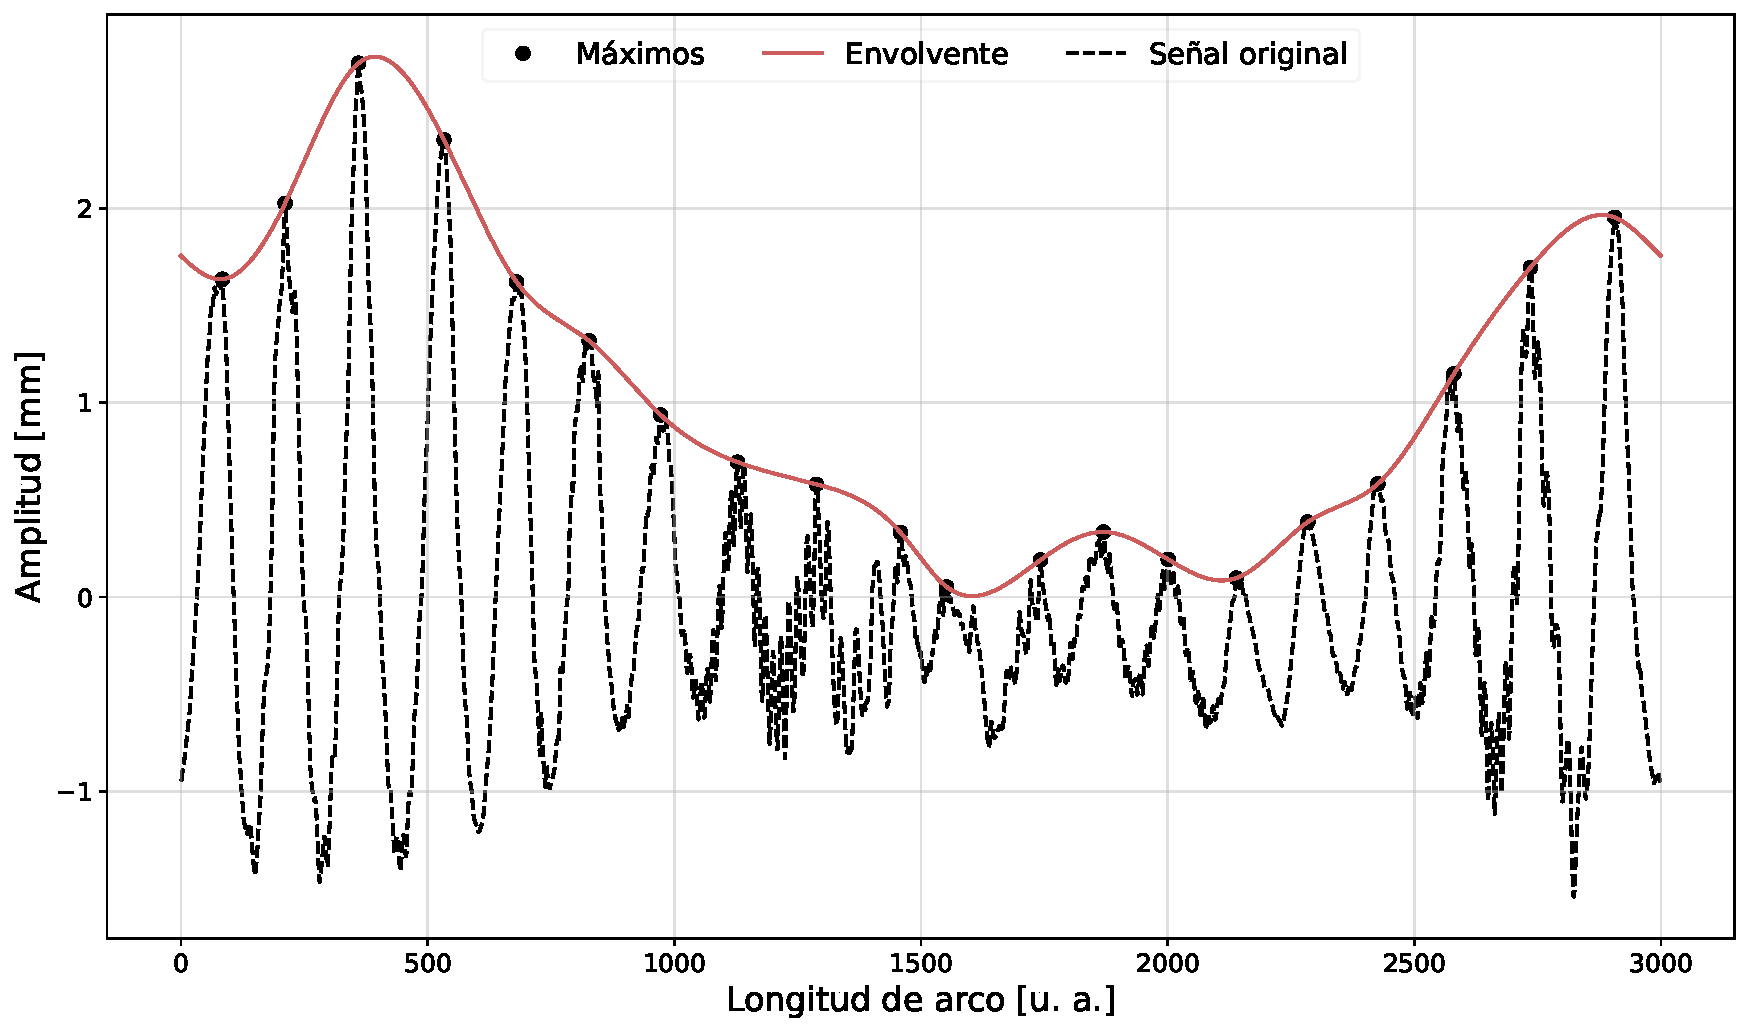
\includegraphics[width=0.9\textwidth]{figs/env_1sample.pdf}
	\end{figure}
	%TODO[berna]: Sacarle el fondo a la legend
\end{frame}

\begin{frame}{Envolvente de la superficie libre}
	\begin{figure}[ht]
		\centering
		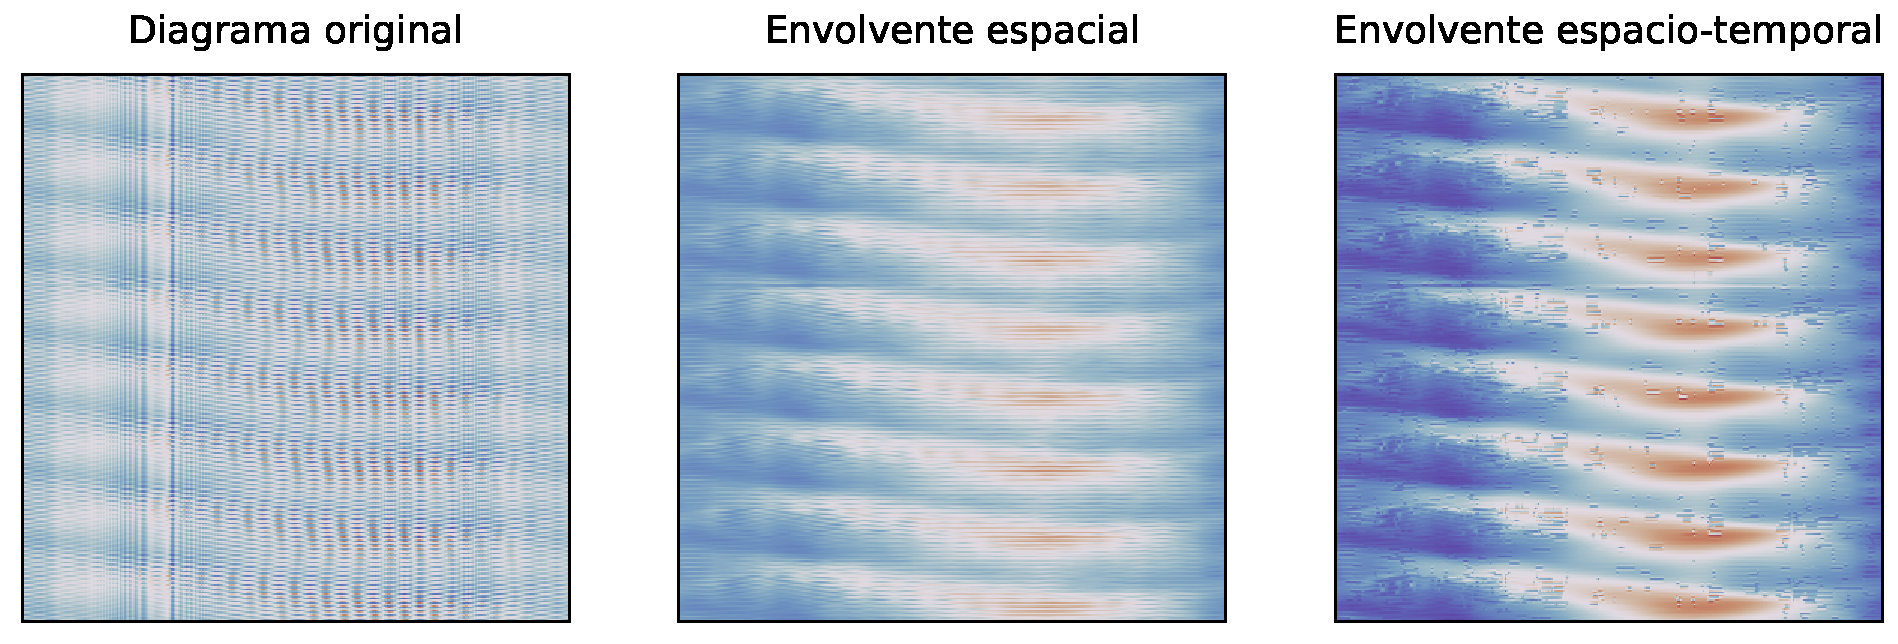
\includegraphics[width=\textwidth]{figs/st_envelopes.pdf}
	\end{figure}
\end{frame}

\section{Perspectivas}
\begin{frame}{Mediciones a analizar}
	\begin{itemize} 
		\item Respuesta del sistema aumentando y disminuyendo la aceleración
			\vspace{0.8cm}
		\item Distribución de la energía en los modos del sistema (con y sin modulación)
			\vspace{0.8cm}
		\item Velocidad característica de los trenes de oscilones
			\vspace{0.8cm}
		\item Ajuste de ecuaciones de amplitud
	\end{itemize}
\end{frame}

\section*{Gracias.}

\section{Diapos que probablemente no usemos}

\begin{frame}{Manejo de archivos y HDF5}
	\begin{figure}[ht]
		\centering
		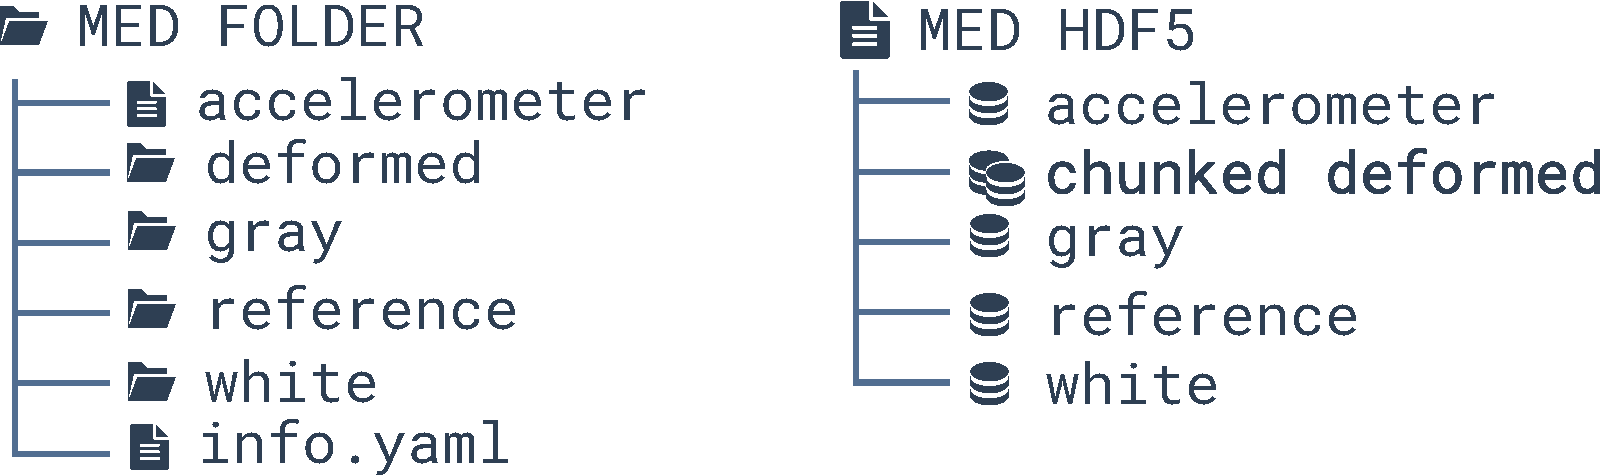
\includegraphics[width=1\textwidth]{figs/med_folder_to_hdf5.pdf}
	\end{figure}
\end{frame}

\begin{frame}{Manejo de archivos y HDF5}
	\begin{figure}[ht]
		\centering
		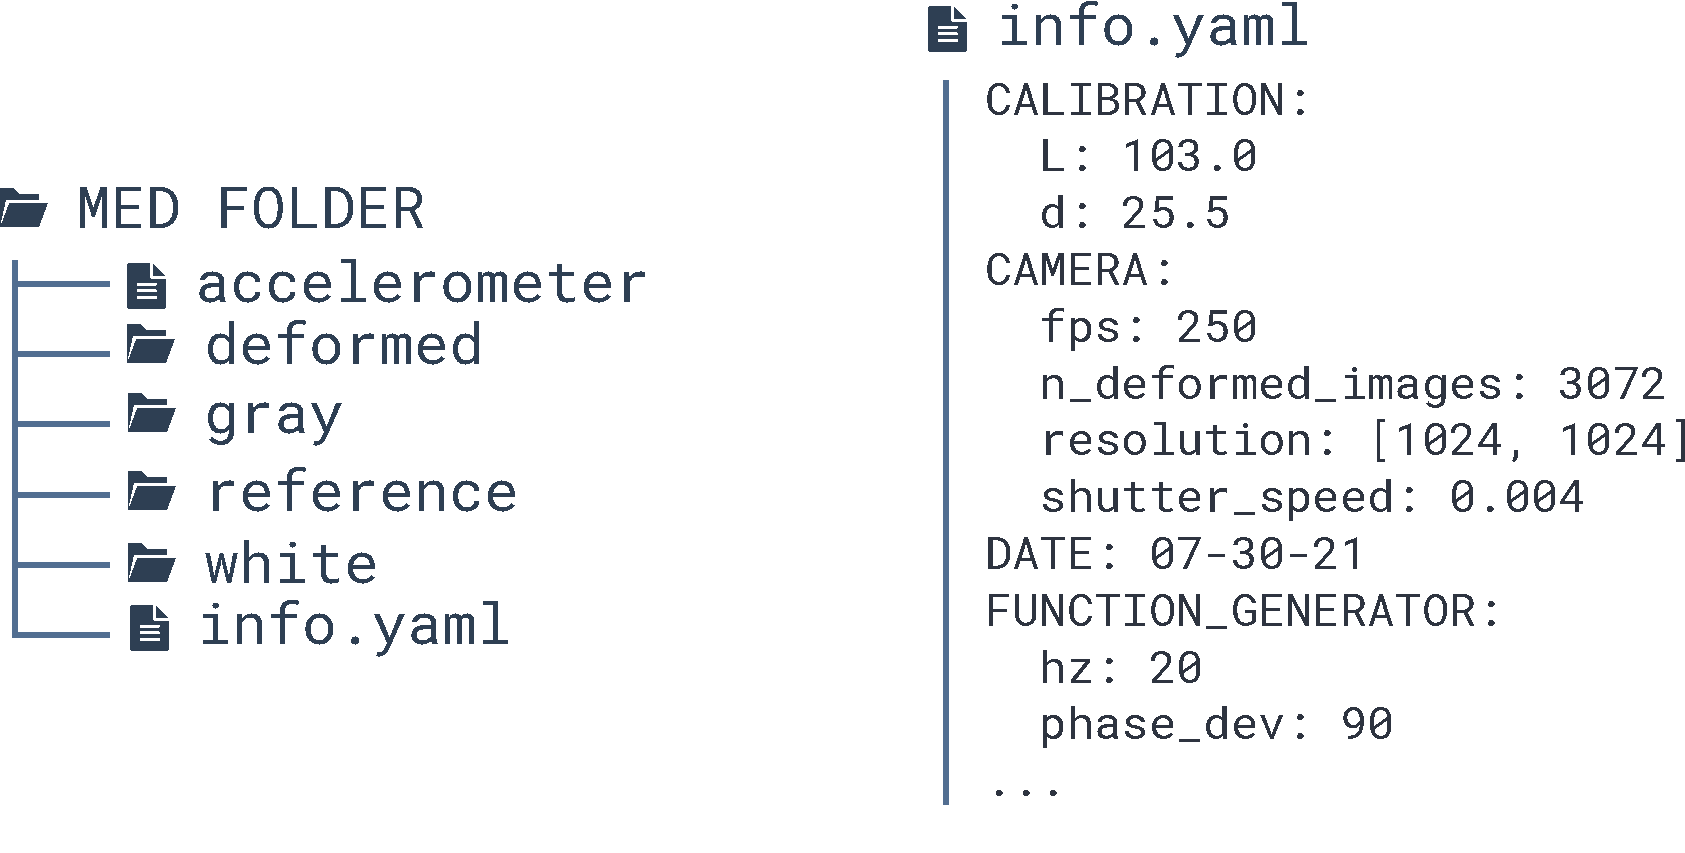
\includegraphics[width=1\textwidth]{figs/med_folder_infoyaml.pdf}
	\end{figure}
\end{frame}

\begin{frame}{HDF5}
	\begin{figure}[ht]
		\centering
		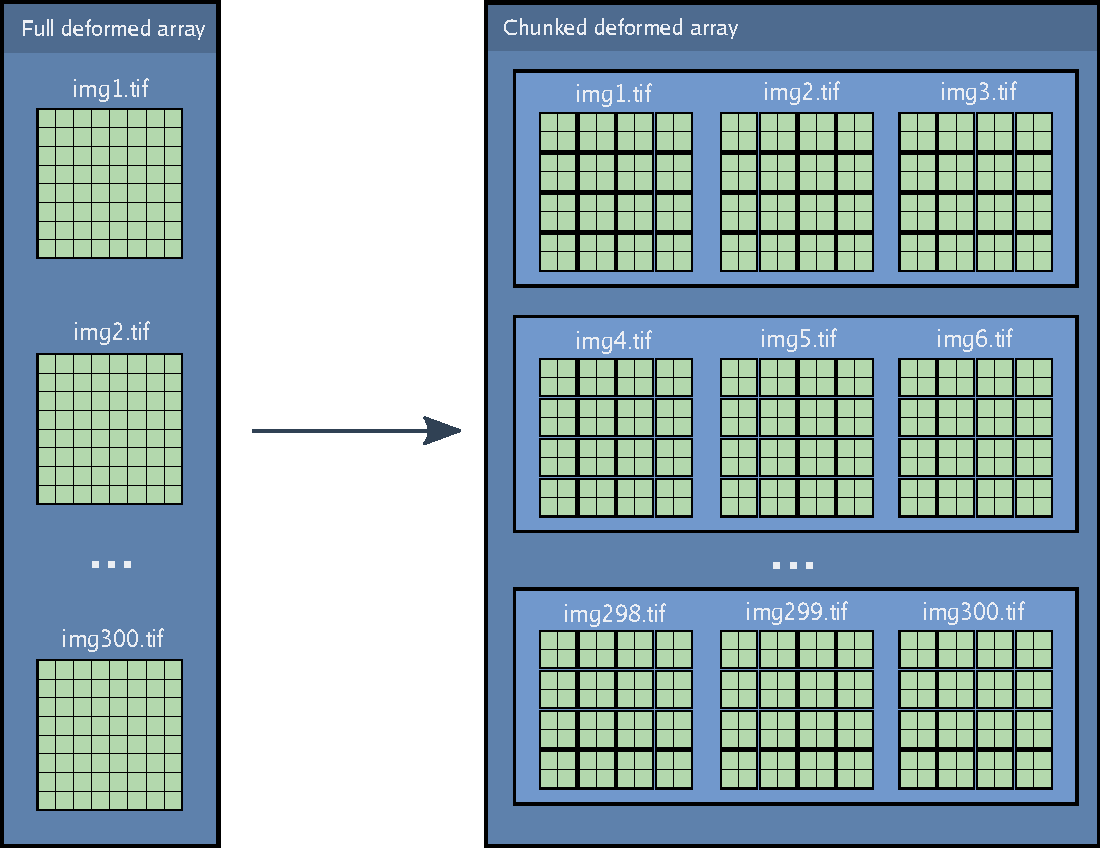
\includegraphics[width=0.7\textwidth]{figs/hdf5_chunk.pdf}
	\end{figure}
\end{frame}



\end{document}
